Tackling the objectives laid out in \cref{sec:navig-virt-subsyst-design} requires an organized and well thought-out plan of work because there are a lot of smaller systems at play that need to work cohesively and synchronously. 




%///////////////////////// # Separation into packages //////////////////////////

The best way to achieve a good plan is by first separating the problem into packages, and in each package have subpackages, each with a collection of modules dedicated to serve a collective purpose in the data treatment and organization chain. 

The system is divided into such packages as follows:

\begin{figure}[H]
	\centering
	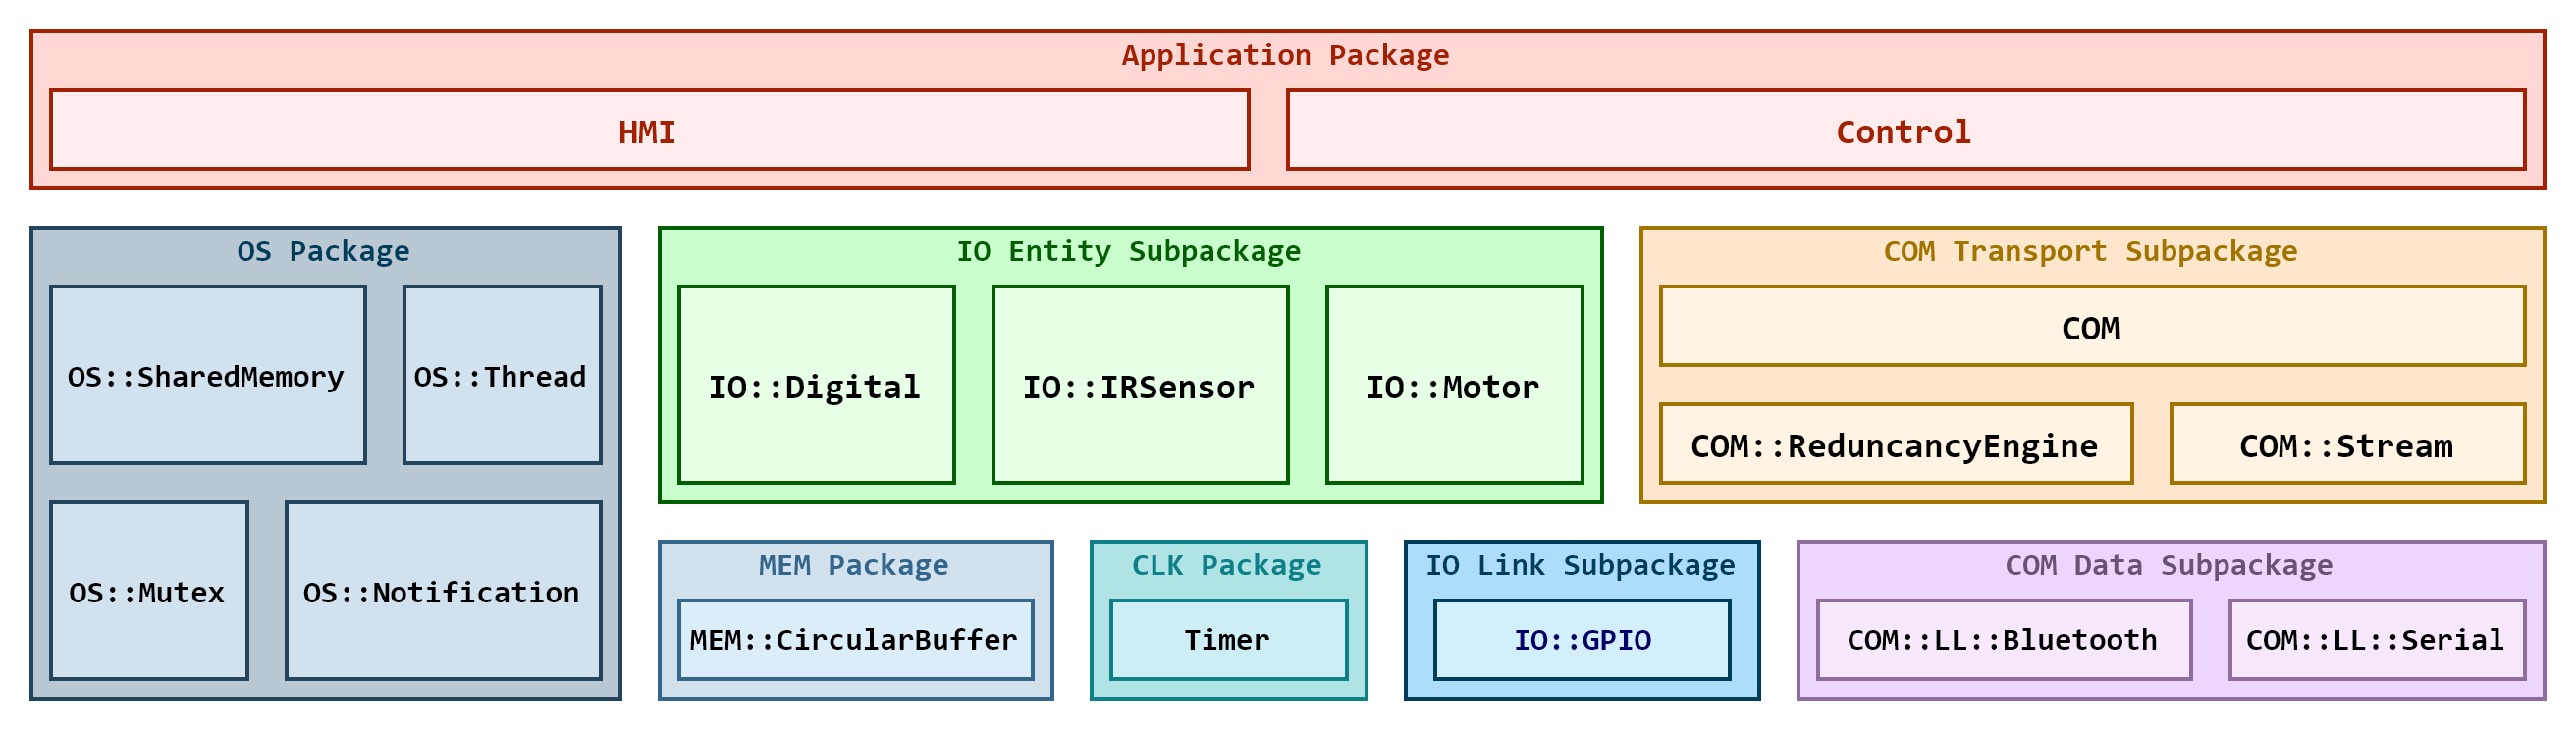
\includegraphics[width=1.0\textwidth]{./img/full-stack-overview.png}
	\caption {Full Stack Overview}
	\label{fig:full-stack-overview}
	\end{figure}
	


%////////////////////////// # Separation into layers ///////////////////////////

Each subpackage also belongs to a certain layer of software, characterized not by the resources it is associated to but by how close the modules within it are to the hardware. Futhermore, the packages should be distributed between layers in such a way that one seldomly need to use another that doesn't belong to the same layer or the layer directly below. 

These layers are, from the bottom to the top:
\begin{itemize}
	\item The High-level Hardware Abstraction Layer, which consists of the \textbf{OS} (partly), \textbf{MEM}, \textbf{CLK}, \textbf{IO Link} and \textbf{COM Data} packages/subpackages. Modules within this layer are responsible for the lower-level interaction with the system's resources so they are made to be thread-safe. Their implementation is platform-dependent and their interface is platform-agnostic. The main goal for this layer of software is to standardize the hardware, making for clean, maintainable and easily portable code. 
	\item The High-level Software Abstraction Layer, consisting of the \textbf{OS} (partly), \textbf{IO Entity} and \textbf{COM Transport} packages. The modules within these packages should serve as an interface with the lower level layer, creating a more intuitive interaction process and mechanisms for processing information asynchronously. This way, when other modules make use of those interfaces, the information is already parsed and ready to be retrieved.\\
	Modules in the layers above ara also highly dependent on both abstraction layers to carry out their tasks in time so the ones in this layer should provide robust mechanisms for exception-handling and timing. 
	\item The Main Application Layer, comprised only of the \textbf{APP} package, where the core functionality lies. As stated earlier, modules in this layer are protected from having to access to most lower-level layers but can use those modules and must use when no other abstraction is provided.
\end{itemize}


%//////////////////////////////// Static model /////////////////////////////////
\subsubsection{Static Model: Package diagram}

\begin{figure}[H]
	\centering
	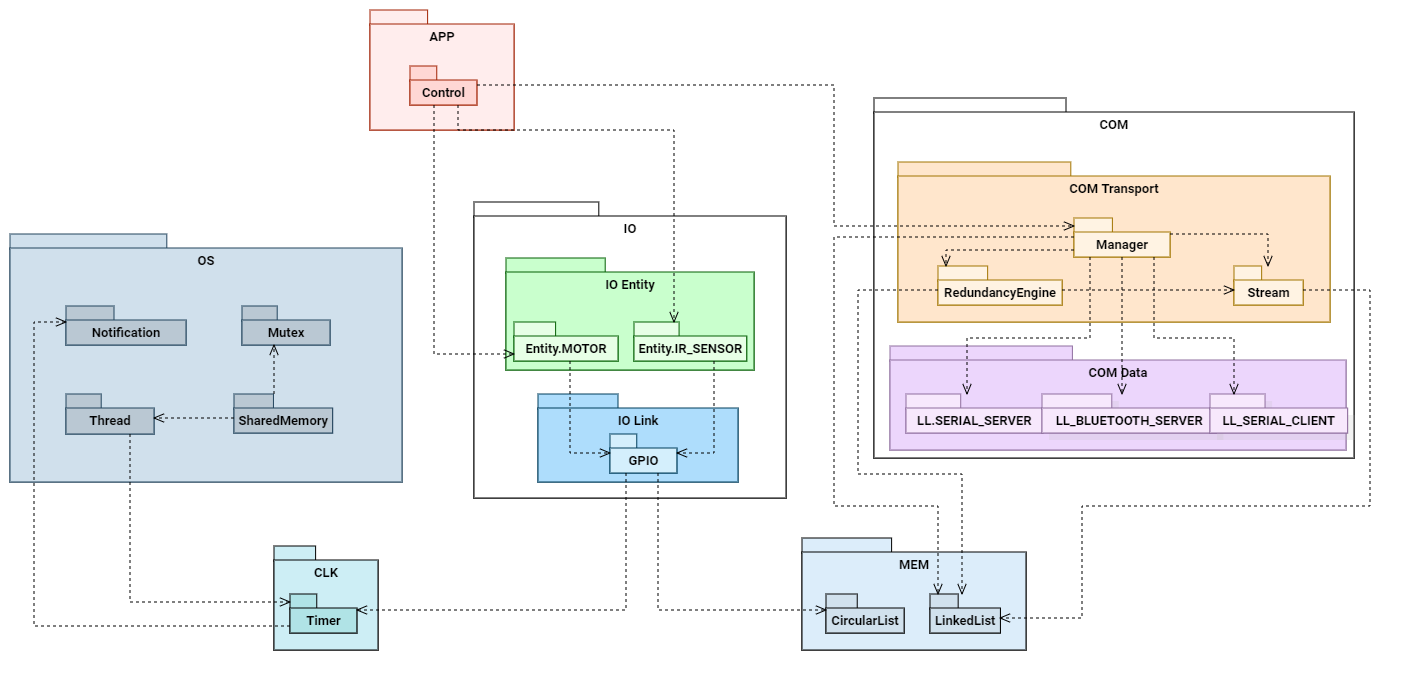
\includegraphics[width=0.8\textwidth]{./img/navig-package-diagram.png}
	\caption {Navigation subsystem package diagram}
	\label{fig:navig-package-diagram}
	\end{figure}



\subsubsection{Static Model: Class diagram}


\begin{figure}[H]
	\centering
	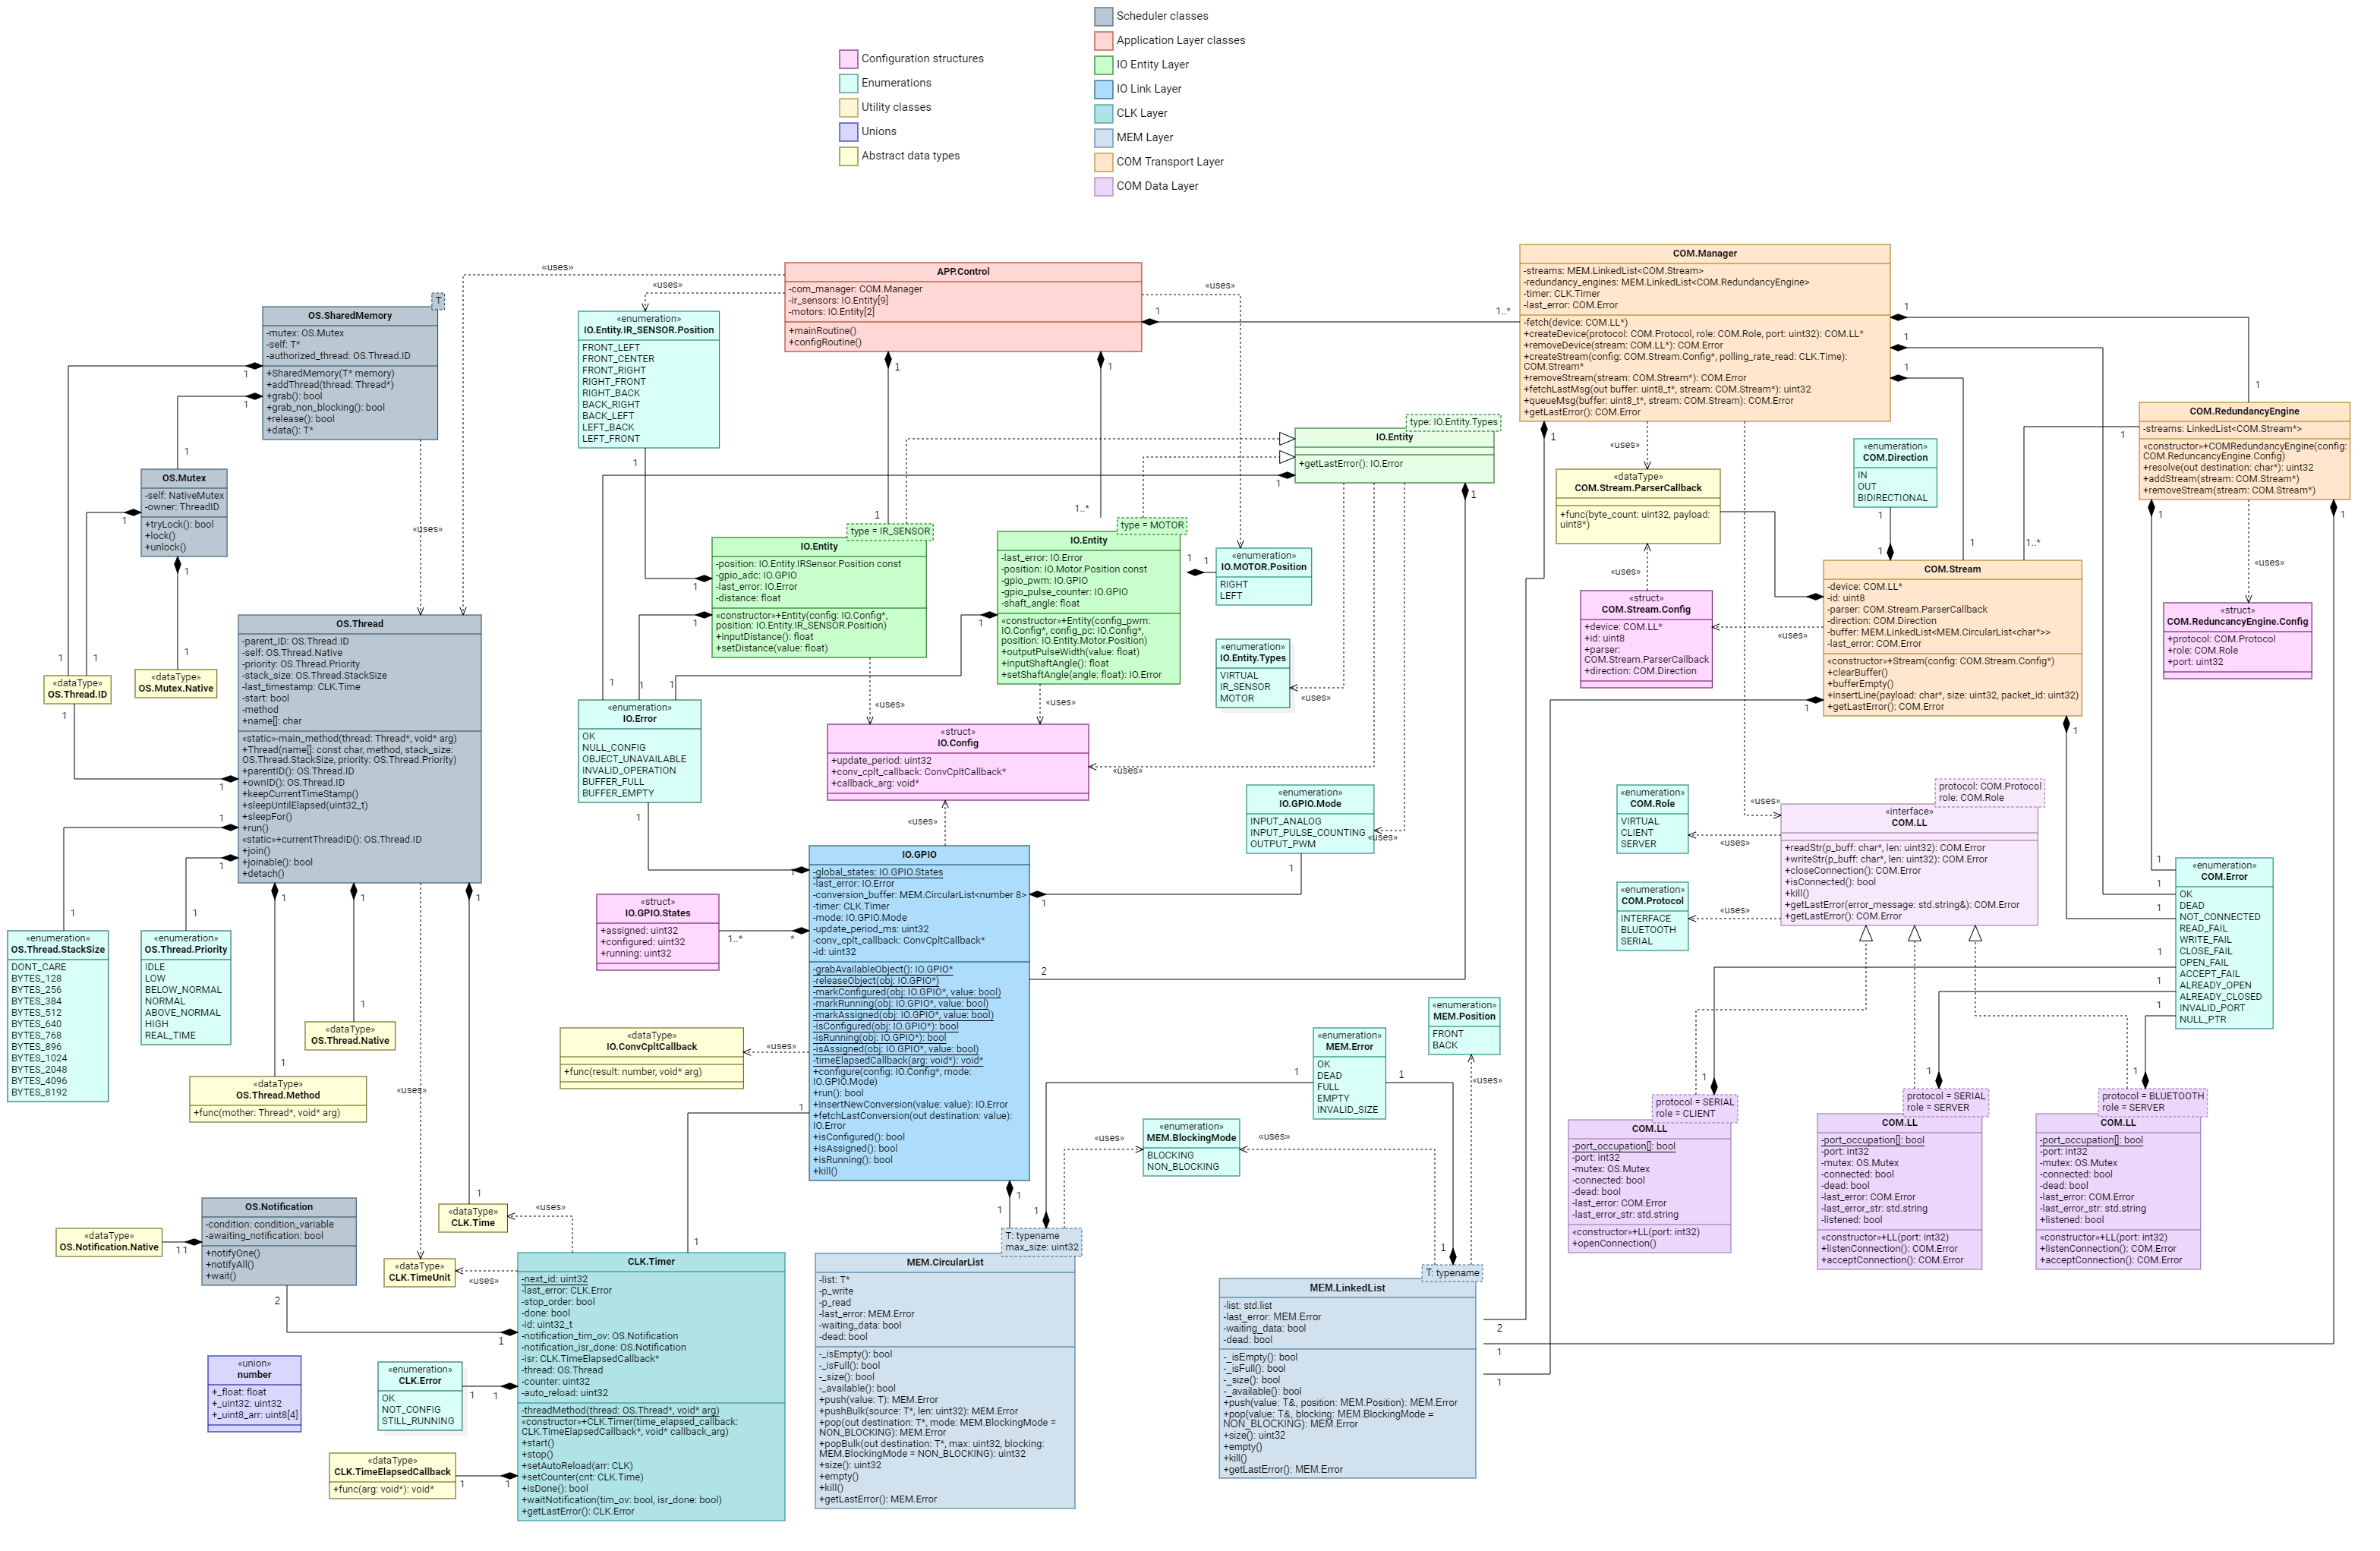
\includegraphics[width=\textwidth]{./img/navig-class-diagram.png}
	\caption {Navigation subsystem class diagram (augmentedin \ref{fig:navig-class-diagram-augmented})}
	\label{fig:navig-class-diagram}
	\end{figure}



%//////////////////////////////// # IO Package /////////////////////////////////
\subsubsection{IO: Input/Output Package}
\label{sec:io-package}
The \textbf{IO} package is comprised of the \textbf{IO Entity} and \textbf{IO Link} subpackages. The modules within these subpackages are the parts of the hardware abstraction layers responsible for standardizing the General Purpose Input/Output resources of the machine.

The \textbf{IO Link} subpackage is the interface provides the most generic yet complete package for interacting with the machine. Its only module \textbf{IO::GPIO} provides such functionality as automatic resource assignment upon creation, automatic buffering of read and output values and the option of executing a specific piece of code when a conversion is completed for better effort distribution between layers.

\begin{figure}[H]
	\centering
	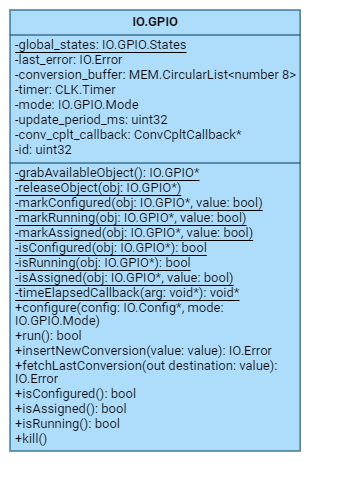
\includegraphics[width=0.38\textwidth]{./img/navig-class-gpio.png}
	\caption {IO::GPIO interface and members}
	\label{fig:navig-class-gpio}
	\end{figure}


The \textbf{IO::Entity} module from the \textbf{IO Entity} subpackage serves for specialization of functionality present in \textbf{IO Link} to serve a certain purpose attached to a physical meaning. This means it also extends the aforementioned callback mechanisms from \textbf{IO::GPIO} for automatic calculation of real-world values based on the measurements taken or otherwise that can be adapted and tailored further to serve the purpose of the specific application. Both provide a modest interface for storing important values calculated in the context of a \texttt{IO::ConversionCpltCallback} and a way to retrieve them.\\

Its \texttt{MOTOR} specialization uses an instance of \textbf{IO::GPIO} as an \texttt{INPUT\_PULSE\_COUNTING} to be able to count the number of pulses from the motor's encoder and output and one as an \texttt{OUTPUT\_PWM} to be able to output a pulse width modulated signal with a duty-cycle $D$ such that 
$$
V_{out average} = \frac{D\times V_{max}}{100}
$$

The \texttt{IR\_SENSOR} specialization uses an instance of \textbf{IO::GPIO} as an \texttt{INPUT\_ANALOG} for application in IR sensing applications. It provides a way to change the last calculated distance specifically for use in the corresponding callback function and an interface for retrieving that same value.

\begin{figure}[H]
	\centering
	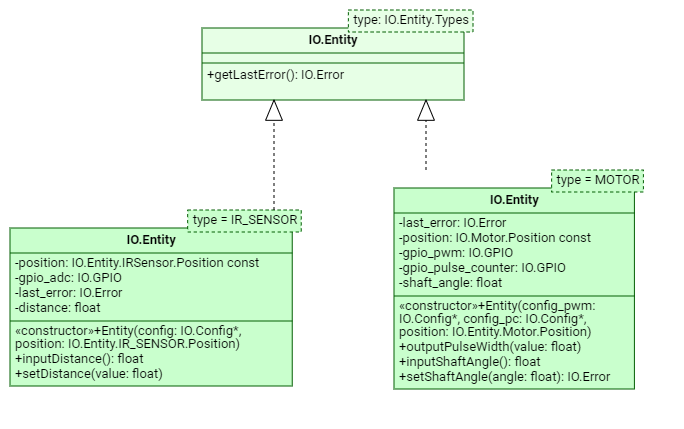
\includegraphics[width=0.65\textwidth]{./img/navig-class-entity.png}
	\caption {IO::Entity interface and specializations' methods and members}
	\label{fig:navig-class-entity}
	\end{figure}



\begin{figure}[H]
	\centering
	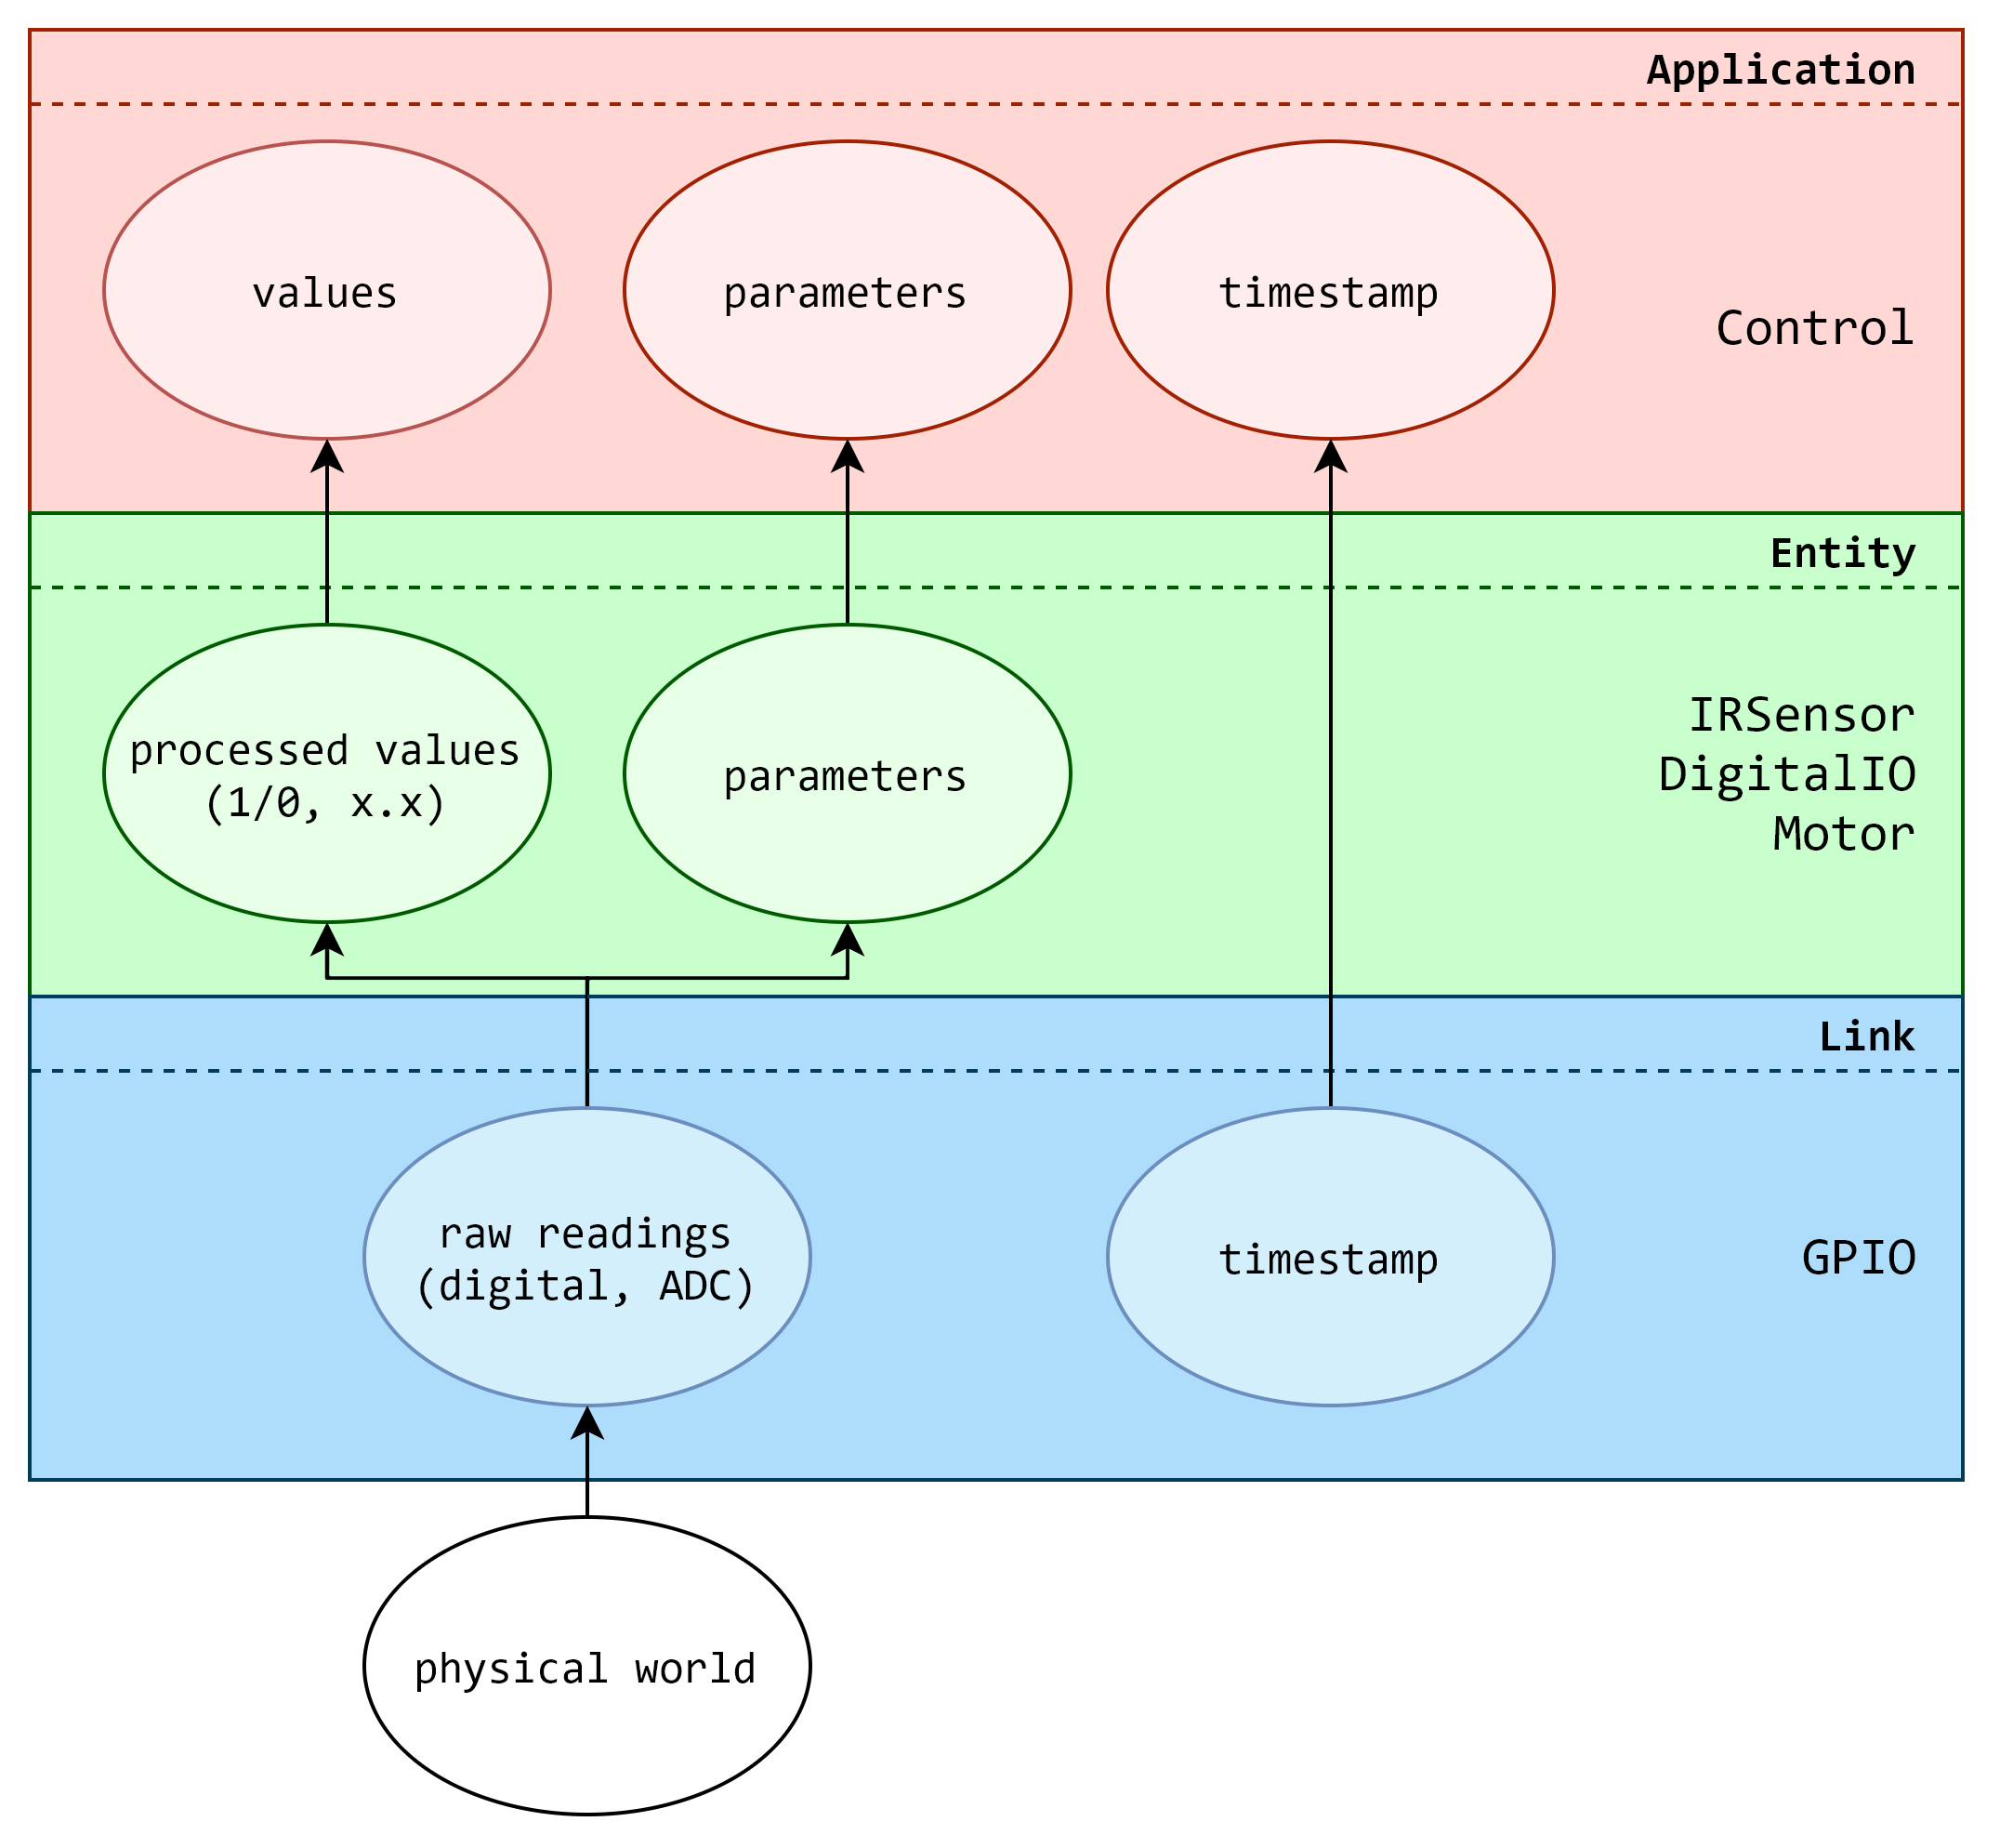
\includegraphics[width=0.5\textwidth]{./img/module-stack-io.png}
	\caption {IO subpackage interaction and information propagation diagram}
	\label{fig:navig-module-stack-io}
	\end{figure}

 


////////////// IMPLEMENTATION
A callback for translating the motor encoder's pulse count into the adequate value of shaft position and rotational velocity. 
A callback for translating the analog value from the IR sensor into the distance from the sensor to an obstacle
/////////////////////////////

%//////////////////////////////// # COM Package ////////////////////////////////
\subsubsection{COM: Communications Package}

The COM package is the sum of the COM Data and COM Transport subpackages. These  modules are responsible for standardizing the access to the inter-device communication resources of each machine. 


The \textbf{COM Data} subpackage is aimed at providing a platform-agnostic interface for communicating over a serial or Bluetooth connection, while also providing specific functionality for different protocols/roles.
The \textbf{COM Transport} subpackage provides tools for managing multiple simultaneous, redundant, multiprotocol and multi-stream connections as well as automatically parsing of data for usage in time-constrained scenarios.

\begin{figure}[H]
	\centering
	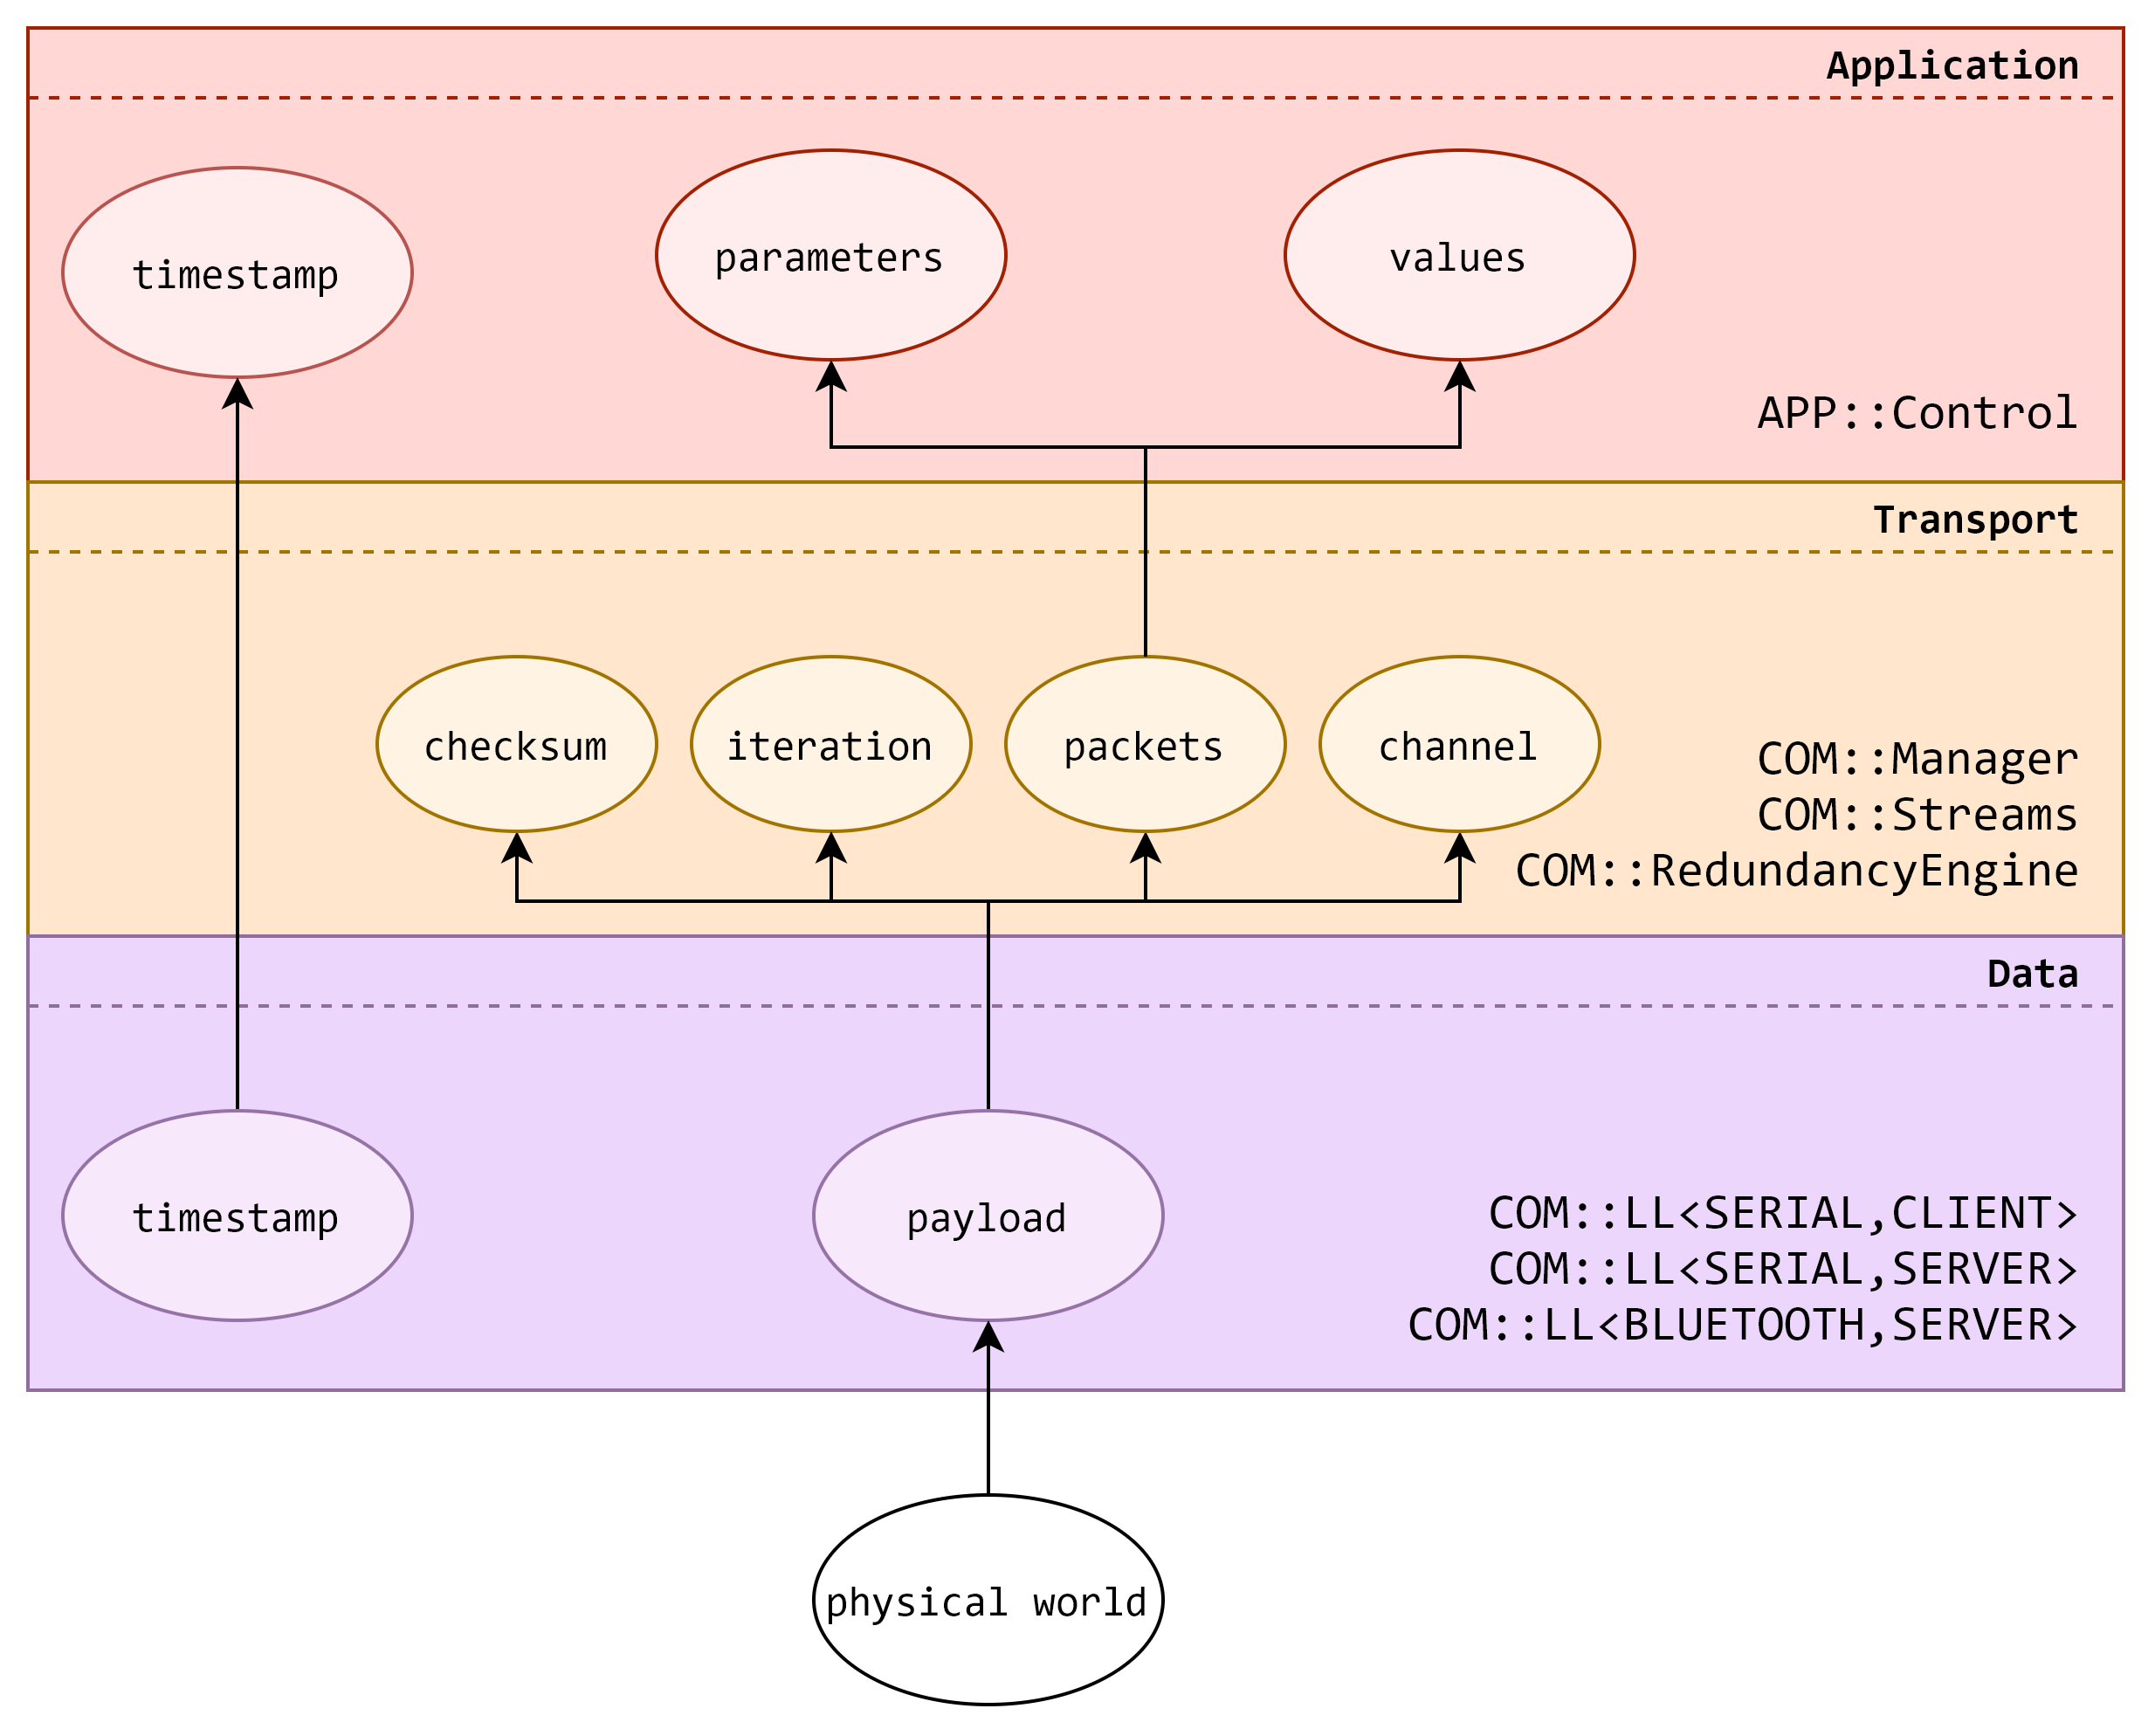
\includegraphics[width=0.5\textwidth]{./img/module-stack-com.png}
	\caption {COM subpackage interaction and information propagation diagram}
	\label{fig:navig-module-stack-com}
	\end{figure}



The \textbf{COM::LL} module 

\begin{figure}[H]
	\centering
	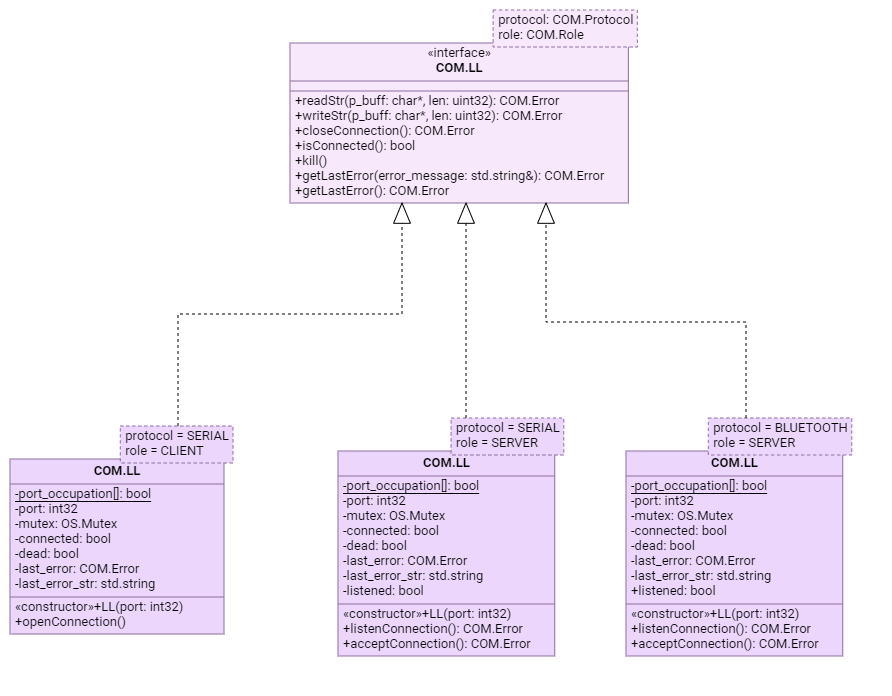
\includegraphics[width=0.8\textwidth]{./img/navig-class-ll.png}
	\caption {COM::LL interface and specializations' methods and members}
	\label{fig:navig-class-ll}
	\end{figure}


The \textbf{COM::Stream} module 

\begin{figure}[H]
	\centering
	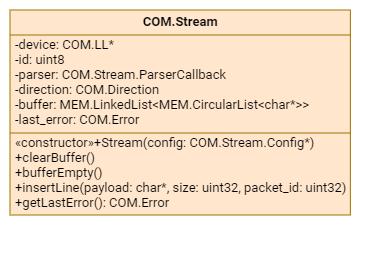
\includegraphics[width=0.4\textwidth]{./img/navig-class-stream.png}
	\caption {COM::Stream interface and members}
	\label{fig:navig-class-stream}
	\end{figure}


The \textbf{COM::RedundancyEngine} module 

\begin{figure}[H]
	\centering
	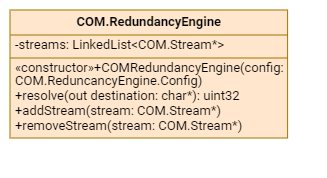
\includegraphics[width=0.35\textwidth]{./img/navig-class-redundancy-engine.png}
	\caption {COM::RedundancyEngine interface and members}
	\label{fig:navig-class-redundancy-engine}
	\end{figure}


The \textbf{COM::Manager} module 
	
\begin{figure}[H]
	\centering
	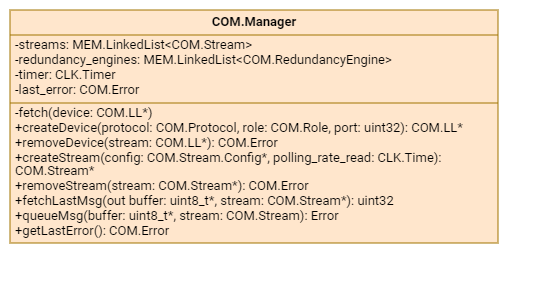
\includegraphics[width=0.5\textwidth]{./img/navig-class-manager.png}
	\caption {COM::Manager interface and members}
	\label{fig:navig-class-manager}
	\end{figure}



%//////////////////////////////// # OS Package /////////////////////////////////
\subsubsection{OS: Scheduler Package}
\label{sec:osPack}
The modules in the \textbf{OS} package mainly serve the purposes of thread creation and management management, inter-thread synchronization and thread-safe access to memory. Therefore, they all revolve around threaded execution although each fills in the need for a special bit of functionality.

The \textbf{OS::Thread} module provides a platform-agnostic interface for creating an object that will use native types and interfaces that allow each object to behave like a separate execution thread. The provided controls for it include execution and sleep mechanisms as well as options for waiting for the end of their execution and detaching threads from the parent thread. Scheduling can be managed with the options concerning thread priority and for the possibility of creating static threads it also provides the chance of delimiting the stack size. 

\begin{figure}[H]
	\centering
	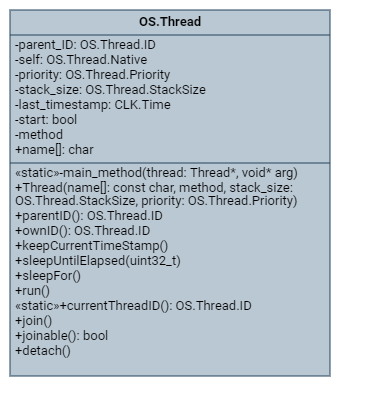
\includegraphics[width=0.4\textwidth]{./img/navig-class-thread.png}
	\caption {OS::Thread interface and members}
	\label{fig:navig-class-thread}
	\end{figure}


The \textbf{OS::Mutex} module provides a way for controlling access to shared resources that are not defined as thread-safe, which is any object that the user might create that is not of any of the modules in the High-level Hardware Abstraction Layer. It can be locked (\texttt{lock()}) in one thread in order to block access to a specific excerpt of code and it can only be locked again by the same thread or any other after it is unlocked (\texttt{unlock()}) by whatever thread locked it. It is thus non-recursive, which means that any thread, including the thread that locked in blocked in the call to \texttt{lock()} it until it is unlocked.

\begin{figure}[H]
	\centering
	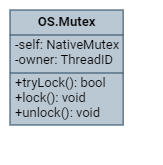
\includegraphics[width=0.15\textwidth]{./img/navig-class-mutex.png}
	\caption {OS::Mutex interface and members}
	\label{fig:navig-class-mutex}
	\end{figure}


The \textbf{OS::SharedMemory} module, one the other hand, provides a platform for sharing resources between specific threads. It may be considered an expansion upon \textbf{OS::Mutex} that is specifically tailored to be used in memory protection and can reduce the roster of threads that get access to a certain memory area. 


\begin{figure}[H]
	\centering
	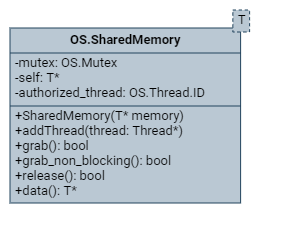
\includegraphics[width=0.25\textwidth]{./img/navig-class-sharedmemory.png}
	\caption {OS::SharedMemory interface and members}
	\label{fig:navig-class-sharedmemory}
	\end{figure}


\textbf{OS::Notification} is a small module that provides the inter-thread synchronization method known as a signal or a notification. A call to \texttt{wait()} from one thread will make it halt until a call for \texttt{notifyOne()} that targets it is given from another thread. A call to \texttt{notifyAll()} will notify all threads. 


\begin{figure}[H]
	\centering
	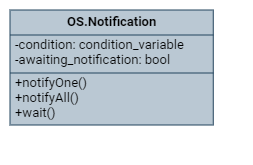
\includegraphics[width=0.28\textwidth]{./img/navig-class-notification.png}
	\caption {OS::Notification interface and members}
	\label{fig:navig-class-notification}
	\end{figure}


\subsubsection{MEM: Memory Structures Package}

The \textbf{MEM} package includes modules that offer typical containers such as linked lists and circular lists that are tightly contained and thread-safe. These are very practical ways of implementing those types of structures in heavily threaded applications as they provide easy-to-use interfaces, low-complexity operations and guarantee safe access to the resources when shared by multiple threads. 
\newline
Both \textbf{MEM::CircularList} and \textbf{MEM::LinkedList} provide interfaces for inserting and removing objects, retrieving basic information about their state, such as their size and a means to empty the list in an efficient fashion. They both also implement the universal error reporting interface with a specific type for such errors, \textbf{MEM::Error}. When making specific operations the user can also choose how the container should react when another thread of execution is accessing the structure: in \textbf{MEM::BlockingMode BLOCKING} mode, the list will wait until the resources are freed and in \textbf{NON\_BLOCKING} mode, in the same situation it will return with an error code.
\newline
The \textbf{MEM::CircularList} provides a medium for creating a fixed-size First-In-First-Out (FIFO) container to which the user can push a single or multiple objects and retrieve them in a similar fashion. 

\begin{figure}[H]
	\centering
	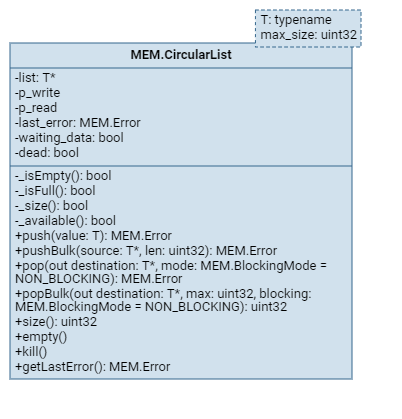
\includegraphics[width=0.4\textwidth]{./img/navig-class-circularlist.png}
	\caption {MEM::CircularList interface and members}
	\label{fig:navig-class-circularlist}
	\end{figure}

The \textbf{MEM::LinkedList} prioritizes quick insertion at the front or the back of any list and removal of specific objects from anywhere in the list with the same complexity. It it optimized exclusively for operations with single objects.

\begin{figure}[H]
	\centering
	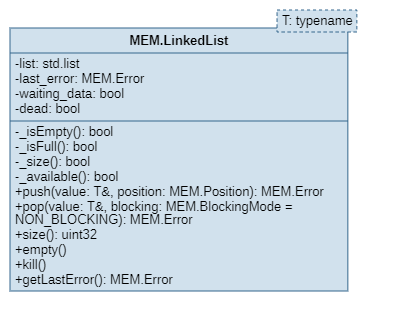
\includegraphics[width=0.4\textwidth]{./img/navig-class-linkedlist.png}
	\caption {MEM::LinkedList interface and members}
	\label{fig:navig-class-linkedlist}
	\end{figure}


The modules within this package are mainly used by the \textbf{IO} and \textbf{COM} class modules for buffering information and storing objects in lists where insertions and removals need to be fast but they can also be used by higher-level classes due to their \textbf{versatile interfaces} and \textbf{general-purpose} nature.

////////////// IMPLEMENTATION
Both lists provide efficient methods for insertion and removal of elements and completely clearing the list, all of these operations with O(1) complexity.
It is implemented with recourse to a C-style array to optimize for use as a single-byte data container (e.g. strings of characters in message buffers).
/////////////////////////////



%//////////////////////////////// # CLK Package ////////////////////////////////

\subsubsection{CLK: Timing Package}

The \textbf{CLK} package is comprised by only the \textbf{Timer} module and convenient type definitions. It provides a means for setting up repeated timed delays and executing a specific routine automatically when each delay ends. It also provides an interface for waiting for the end of the timed delay and/or the execution of the specified routine and autonomously notifies all waiting objects of these events.
It is mainly used by the \textbf{IO::GPIO} class for timing conversions but it can as easily be used by higher-level classes due to its \textbf{versatile interface} and \textbf{general-purpose} nature.

\begin{figure}[H]
	\centering
	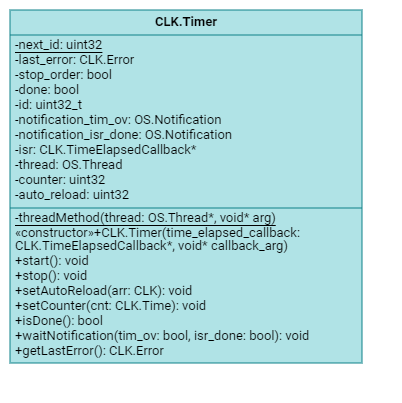
\includegraphics[width=0.43\textwidth]{./img/navig-class-timer.png}
	\caption {CLK::Timer interface and members}
	\label{fig:navig-class-timer}
	\end{figure}



%//////////////////////////////// # APP Package ////////////////////////////////

\subsubsection{APP: Main Application Package}

The main application package is comprised by  

